\section{Tasas de interés e instrumentos derivados}

%----------------------------------------------------------------------------------------

\begin{frame}
    \frametitle{Tasa de interés simple}
    Sean A y B dos contrapartes, tal que A le presta un monto \$1 en tiempo $T_1$ a B y B le paga un monto \$1 en tiempo $T_2$ más cierto interés K entre $T_1$ y $T_2$. 
    \begin{figure}[h]
       \centering
       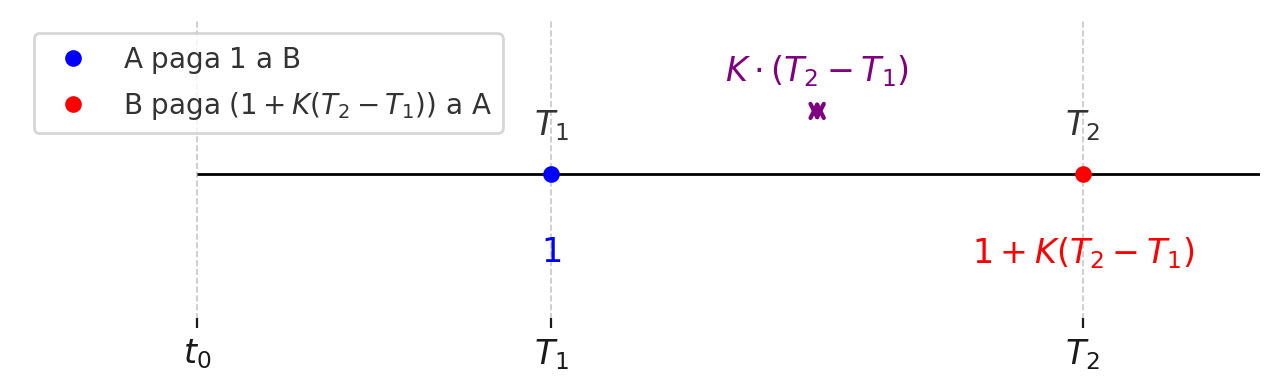
\includegraphics[width=\textwidth]{img/cap1/accrual_simple.png}
       \caption{Tasa simple}
       \label{accrual_simple}
   \end{figure}
\end{frame}

%----------------------------------------------------------------------------------------

\begin{frame}
    \frametitle{Sistemas de Capitalización}
    \begin{itemize}
        \item \textbf{Capitalización Simple:} El interés se calcula sobre el capital inicial. Un interés de \$100 a una tasa de 10\% anual durante 3 años resulta en $100 \times (1+0.1 \times 3) = 130$.
        \item \textbf{Capitalización Compuesta Discreta:} El interés se calcula sobre el capital inicial más los intereses acumulados. Invertir \$100 a una tasa de 10\% anual durante 3 años con capitalización semestral resulta en $100 \times (1+0.1/2)^{2 \times 3} = 133.1$.  
        \item \textbf{Capitalización Compuesta Continua:} El interés se calcula sobre el capital inicial más los intereses acumulados, pero en un límite continuo. Invertir \$100 a una tasa de 10\% anual durante 3 años con capitalización continua resulta en $100 \times e^{0.1 \times 3} = 134.98$. 
    \end{itemize}

\end{frame}

%----------------------------------------------------------------------------------------

\begin{frame}
    \frametitle{Bonos cupon cero}
    Componentes:
    \begin{itemize}
        \item \textbf{Valor nominal (N):} Monto a pagar al vencimiento.
        \item \textbf{Tasa de interés (r):} Tasa \textit{cero}.
        \item \textbf{Tiempo hasta el vencimiento (T):} Tiempo en años hasta el vencimiento.
        \item \textbf{Precio (P):} Precio actual del bono.
    \end{itemize}
    % side by side equations
    \begin{columns}
        \column{0.4\textwidth}
            \begin{equation*}
                P = \frac{N}{(1+r)^T}
            \end{equation*}
        \column{0.4\textwidth}
            \begin{equation*}
                P = N \cdot e^{-rT}
            \end{equation*}
    \end{columns}
\end{frame}

%----------------------------------------------------------------------------------------

\begin{frame}
    \frametitle{Valoración de un bono con cupones}
    Consideremos un bono de principal \$100, madurez en 2 años y tasa cupón 5\% semianual.\\
    Supongamos que las tasas cero a 6 meses, 1 año, 1.5 años y 2 años son 4\%, 4.5\%, 5\% y 5.5\% respectivamente.\\
    \begin{itemize}
        \item \textbf{Flujos de caja:} \$2.5, \$2.5, \$2.5, \$102.5
        \item \textbf{Tasas cero:} 4\%, 4.5\%, 5\%, 5.5\%
        \item \textbf{Precios:} $\$2.5 \cdot e^{-0.04 \cdot 0.5} + \$2.5 \cdot e^{-0.045 \cdot 1} + \$2.5 \cdot e^{-0.05 \cdot 1.5} + \$102.5 \cdot e^{-0.055 \cdot 2}$
        \item \textbf{Precio total:} 98.98
    \end{itemize}
\end{frame}
%----------------------------------------------------------------------------------------

\begin{frame}
    \begin{figure}[h]
       \centering
       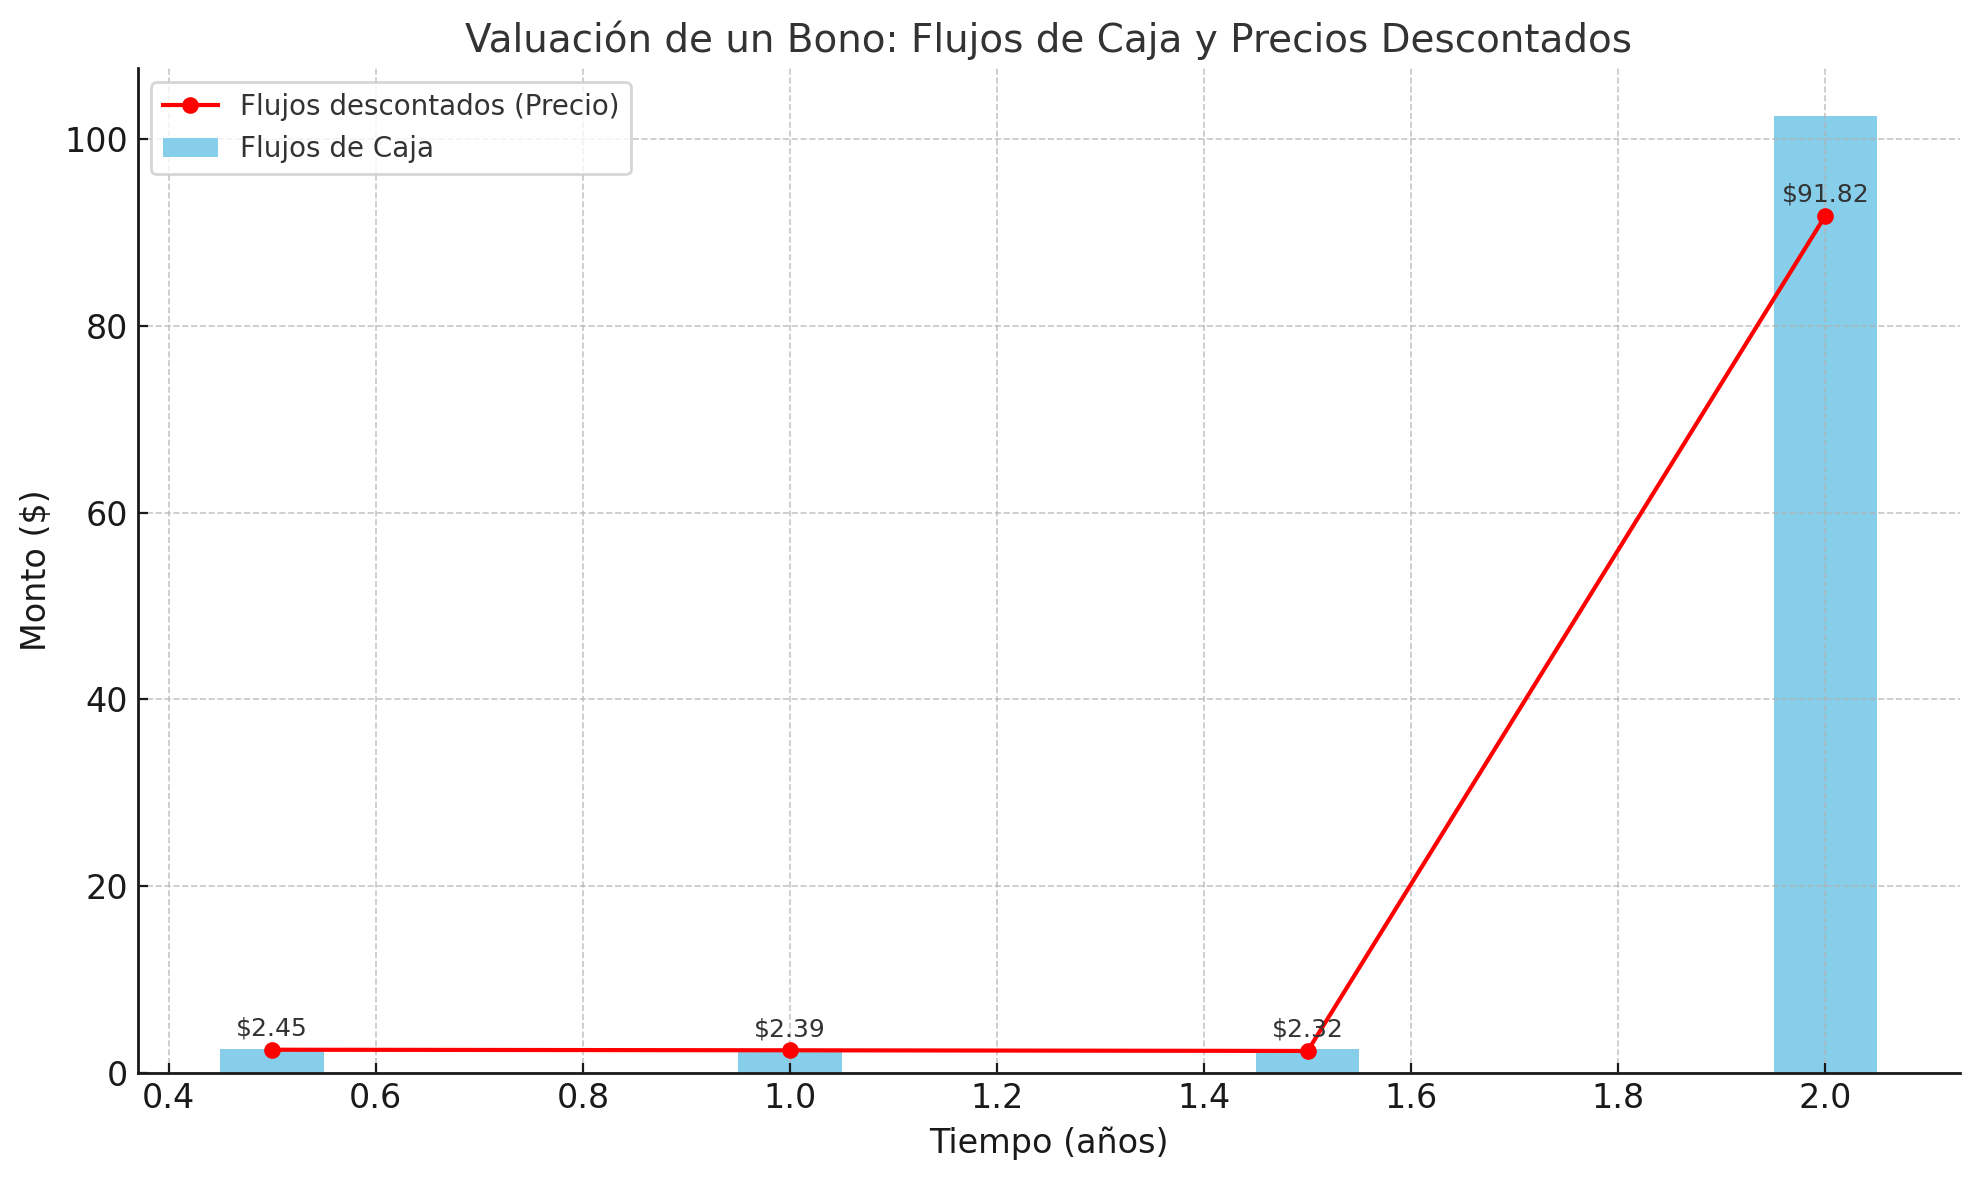
\includegraphics[width=\textwidth]{img/cap1/bono_cupon.jpg}
       \caption{Valoración de un bono con cupones}
       \label{bono_cupon}
   \end{figure}
\end{frame}
%----------------------------------------------------------------------------------------